\chapter{BELL INEQUALITY}

\section{Bell's Theorem and the Non-Locality of the universe}

This dates back to 1935, when Albert Einstein and his colleagues Boris Podolsky and Nathan Rosen together published a paper named \textquote{\textbf{Can Quantum-Mechanical Description of Physical Reality be Considered Complete?}}\cite{EPR_Paradox}

\subsection{\acs{EPR} Paradox}

The fundamental conclusion reached in the paper\cite{EPR_Paradox} authored by Einstein and his colleagues was not that quantum mechanics are erroneous in terms of making predictions that contradict observations or experiments. Instead, they asserted that the reality depicted by quantum mechanics is an incomplete portrayal of reality. They contended that a more profound explanation must exist, even though they were unable to provide such an explanation. They believed that the paper established the necessity of uncovering this deeper understanding.

Their analysis was based on the concept of quantum entanglement, which is illustrated by the idea that two particles can be widely separated and yet exhibit a connection as if there is an invisible quantum mechanical thread that links them together.

\begin{figure}[htbp]
	\centering
	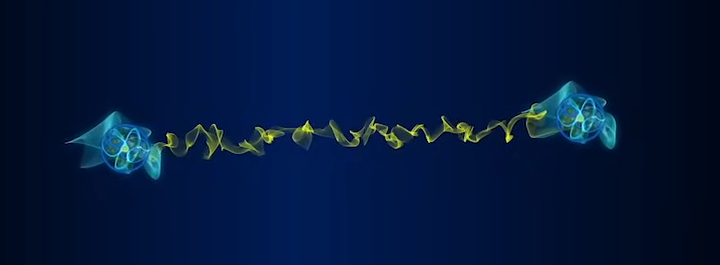
\includegraphics[width=0.70\textwidth]{gfx/diagrams/Entaglement.png}
	\caption{Pictorial representation of quantum entangled particles\cite{worldsciencefestival2024}}
	\label{fig:3.1}
\end{figure}

In standard quantum mechanics, entangled particles exhibit a phenomenon where a change in one particle, for example the one on the right, can immediately impact the measurement of the particle on the left, despite being separated by significant distances. This behavior, characterized by Einstein as \textquote{\textbf{Spooky action at a distance}}, presents a peculiar and intriguing aspect of quantum mechanics.

Let's delve further into the \acs{EPR} paradox and explore the points of contention that Einstein and others had regarding the quantum mechanical spin of particles. We can imagine that we have a couple of detectors and one detector on the right, one detected on the left and in the middle there is a device that will send out particles that are entangled.  

\begin{figure}[htbp]
	\centering
	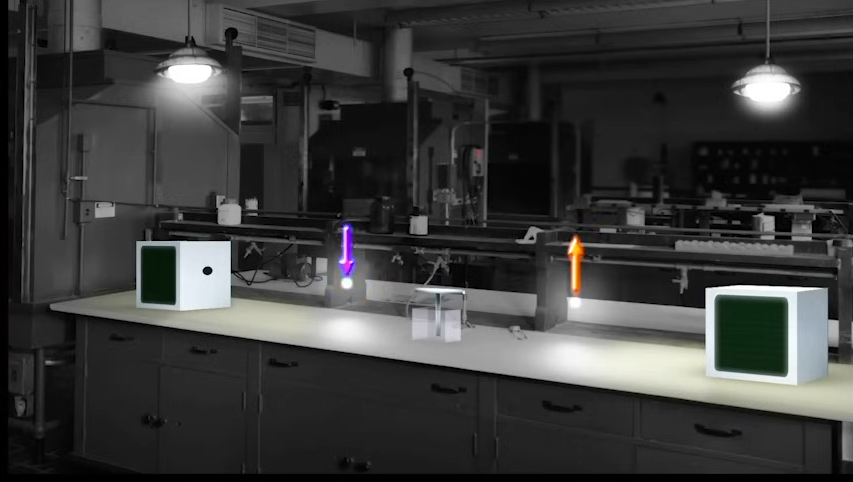
\includegraphics[width=0.70\textwidth]{gfx/diagrams/Entaglement_Measurement(a).png}
	\caption{Pictorial representation of a lab generating two entangled particle with  opposite spin \cite{worldsciencefestival2024}} 
	\label{fig:3.2}
\end{figure}

Now when these entangled pairs reach the detectors, the actual measurement of their spin is calculated. The spookiness is that according to quantum mechanics, the particles are always in a fuzzy mixture of spin orientation and yet upon measurement they both disambiguate that both choose a definite reality even though they're far apart, they're somehow able to correlate the outcomes.If one particle is found to be spin up upon measurement, its entangled counterpart inevitably displays spin down, and vice versa.

Einstein contended that particles do not exist in a state of ambiguous up-and-down spin until they reach the detectors, only when measured do they definitively assume a particular state. He argued that this implied some sort of mysterious interaction between these widely separated particles, which he believed was not how the world functioned. According to Einstein, if a detector detects a particle as spinning up, then it always was spinning up; it never existed in the indeterminate state depicted by the mathematics of quantum mechanics. Consequently, the trio asserted in their paper\cite{EPR_Paradox} that the mathematics of quantum mechanics is incapable of providing a complete and comprehensive description of reality.

\subsection{John Bell's Experimental Proof Validates Einstein's View of Reality}

\begin{figure}[htbp]
	\centering
	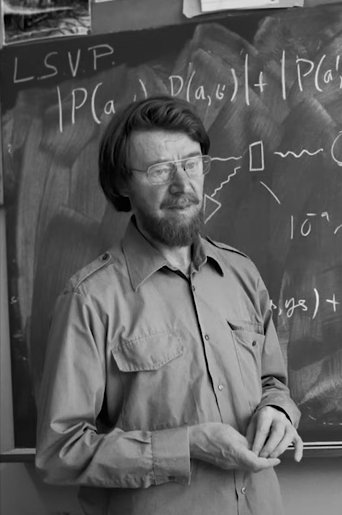
\includegraphics[width=0.35\textwidth]{gfx/diagrams/John_Bell.png}
	\caption{John Bell \cite{worldsciencefestival2024}}
	\label{fig:3.3}
\end{figure}

In 1964, John Stuart bell, a physicist from Northern Ireland, authored a paper\cite{Bell_Paper} entitled \textquote{\textbf{ON THE EINSTEIN PODOLSKY ROSEN PARADOX}}. He writes in his paper\cite{Bell_Paper} that shows the Einstein's view of reality, in which particles are always definite that yields a measurable difference is testable. 

Let us consider the previous experiment with two detectors and a device that send out entangled particles. But this time we are using an upgraded detectors.i.e., they don't just measure the spin along one axis, but these can measure the particle spin about three different axes that are 120° from each other. According to Einstein's perspective on reality, particles inherently possess a fixed value, more like a concealed value even before measurement. This concept is widely known as local realism. Embracing the local realism phenomenon, particles are required to have specific spins along all three possible axes.

\begin{figure}[htbp]
	\centering
	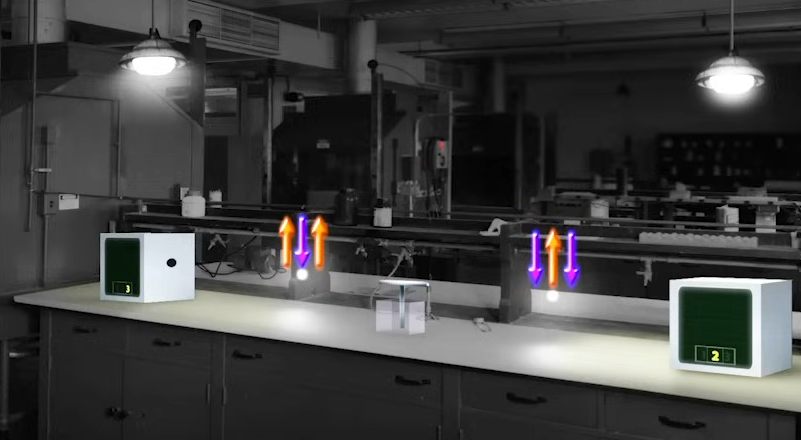
\includegraphics[width=0.70\textwidth]{gfx/diagrams/Entanglement_Measurement(b).png}
	\caption{Spin Measurement in 3 different Axes of the Entangled pairs\cite{worldsciencefestival2024}}
	\label{fig:3.4}
\end{figure}

There is now the possibility of measuring the same spin in the detectors when measured at two different axis. For instance, if the first entangled particle is measured on axis 1, a spin up is obtained at the left detector and likewise, a spin up is obtained at the right detector when measured on axis 2. Bell argues that if this experiment is repeatedly carried out with the detector settings being randomly selected for each trial, the instances where, the detectors register opposite spins will occur at least 5/9 of the time in the overall outcomes. In the given scenario, there are clearly 9 potential results, and the spins are opposite in 5 out of 9 occurrences.

In the context of two particles and three axes, it is reasonable to deduce that at least two of the spin directions must be identical. There are scenarios where all three axes share the same spin orientation (such as up, up, up on the left particle and down, down, down on the right particle). In this particular scenario, all 9 outcomes yield opposite spin results for 9 possible measures. Thus, the probability of the result indicating opposite spins is five out of nine when all the spins along the three axes are not the same and nine out of nine when they are the same.

\begin{figure}[htbp]
	\centering
	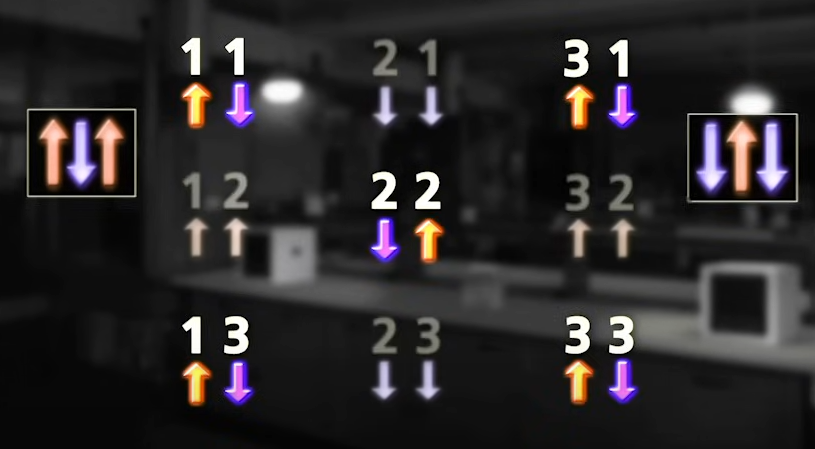
\includegraphics[width=0.70\textwidth]{gfx/diagrams/possible_outcomes.png}
	\caption{Possible outcomes of the spin measurement\cite{worldsciencefestival2024}}
	\label{fig:3.5}
\end{figure}

In repeated experiments involving random entangled particles and random detector settings conducted over a large number of iterations, it is expected that at least 5 out of 9 times, or approximately 55\% of the time, opposite spin results will be obtained. This aligns with Einstein's belief that particles possess definite spins before measurement. However, empirical evidence suggests that the frequency of obtaining opposite spins is considerably lower, around 50\%, contradicting Einstein's perspective. Instead, this outcome supports the standard quantum mechanics calculation, which indicates that particles exist in a nebulous combination of spin states rather than in a predetermined state.

The whole idea behind EPR Paradox and Einstein's view of hidden variables theory was to rule out the \textquote{\textbf{Spooky action}} in between and non-locality. However, the results of experiments suggest otherwise.

\section{Quantenkoffer - Quantum Science Suitcase}

The Quantenkoffer, an innovative device, designed and developed by qutools GmbH, serves as a portable and user-friendly quantum photonics laboratory for conducting a wide range of experiments spanning a century of quantum physics. Its primary strength lies in its adaptability to both generate and detect visible laser light, single photons, and even entangled pairs. This is made possible through the integration of optical elements, mechanical components, and digital circuits, enabling a comprehensive coverage of experiments and topics within the realm of quantum physics.

\begin{figure}[htbp]
	\centering
	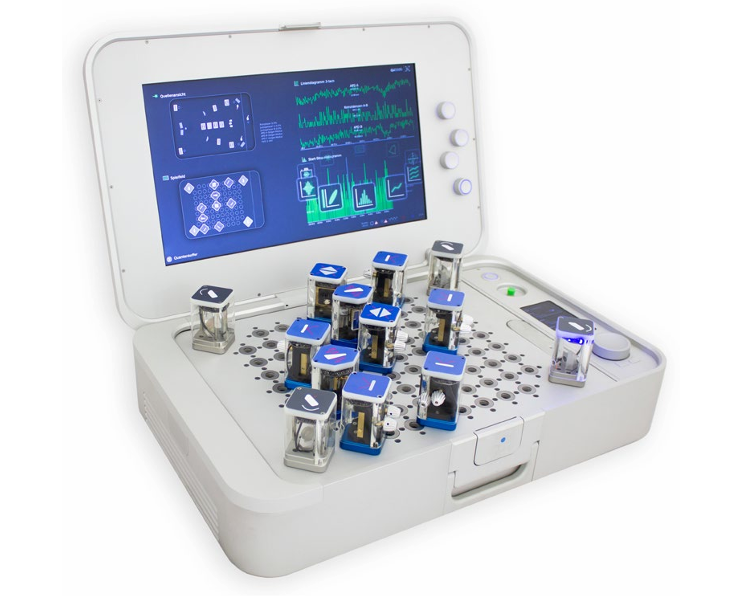
\includegraphics[width=0.60\textwidth]{gfx/diagrams/QuantenKoffer.png}
	\caption{Quantenkoffer\cite{quantenkoffer}} 
	\label{fig:3.6}
\end{figure}

\section*{The Key features of the Quantenkoffer \cite{quantenkoffer}:} 

\begin{itemize}
	\item \textbf{Experiment Flexibility}: On the high-precision board with 86 slots various setups can be individually created by placing the optical tokens into the electromechanical slots. Conducting well-known photonics experiments or setting up new ones can be as easy as playing. 
	
	\item \textbf{Motorized Adjustment:}  The possible automatic adjustment through actuators and sensors facilitates the setup of experiments and the quick realization of measurements, allowing for the playful immersion into the fascinating world of quanta.

	\item \textbf{Single Photons, Entangled Pairs: } A set of lasers and optical crystals form the core of the photon source, which the user can view by flipping the optical setup board. Single pairs of photons are generated through nonlinear processes within optical crystals. Each element of the precise source can be adjusted by the user or automatically optimized by the Quantenkoffer. Additional red laser light follows the path of the single photons for proper adjustment of the optical setups.

\begin{figure}[htbp]
	\centering
	\includegraphics[width=0.60\textwidth]{gfx/diagrams/QuantenKoffer(b).png}
	\caption{Quantenkoffer(b)\cite{quantenkoffer}} 
	\label{fig:3.7}
\end{figure}

	\item \textbf{Intuitive Operation} After the automatic detection of the inserted tokens, a setup display appears on the touch-pad. The user-friendly software supports the user in choosing from a wide range of display-widgets, four of which are active on the large monitor.

	\item \textbf{Picosecond Range Timing: } The ultra-fast processing of the measured events, enabled through powerful digital technology, allows the detection of time differences in the picosecond range, for example to measure the speed of light on the board with few tokens.

	\item \textbf{Optical Tokens - the quBricks: } A variety of optical tokens can be placed on the high-precision board and used in different experiments. The Quantenkoffer identifies, reads, and digitally manages the markers through the electronics surrounding the partially motorized optical elements. Additionally, a touch sensor on top of each quBrick adds physical engagement to enhance cognitive activation during the learning process.
	
	\begin{figure}[htbp]
		\centering
		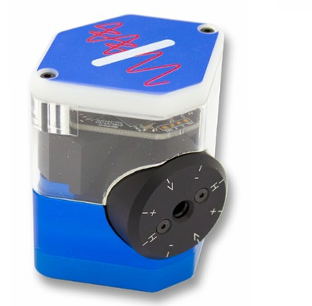
\includegraphics[width=0.40\textwidth]{gfx/diagrams/quBricks.png}
		\caption{quBricks\cite{quantenkoffer}} 
		\label{fig:3.8}
	\end{figure}
	
\end{itemize}

\section{Realization of Bell's Inequality with the Quantenkoffer}

\subsection{Theoretical background}
\label{sec:theoretical_background}

The most widely used version of Bell's inequality in experimental tests is the one formulated by Clauser, Horne, Shimony, and Holt (referred to as \acs{CHSH}). The key concept behind the \acs{CHSH}-Bell inequality is that in local realistic theories, the absolute value of a specific combination of correlations between two particles is constrained by 2. The inequality can be expressed as:
$$ S(\alpha, \alpha', \beta, \beta') = [E(\alpha, \beta) + E(\alpha', \beta) - E(\alpha, \beta') + E(\alpha', \beta')] \leq 2$$ 
where $\alpha(\alpha')$ and $\beta(\beta')$ denote the local measurement settings of two observers, each receiving one of the particles. 


The coincidence count rate for the combination of polarizer settings $C(\alpha,\beta)$ is defined, and the normalized expectation value $E(\alpha,\beta)$ of the correlations between the measurements is given by: 
$$ \frac{C(\alpha,\beta) - C(\alpha,\beta_p) - C(\alpha_p,\beta) + C(\alpha_p,\beta_p)}{C(\alpha,\beta) + C(\alpha,\beta_p) + C(\alpha_p,\beta) + C(\alpha_p,\beta_p)} $$
where $\alpha_p$ and $\beta_p$ are the polarization perpendicular - that is rotated by $90\degree$ - with respect to $\alpha$ and $\beta$.

Measurements of the coincidence count rate with entangled photons reveal a sinusoidal dependence, described by $ C(\alpha,\beta ) \propto cos 2(\theta)$, where $\theta$ is the angle difference between the polarizer orientations. This behavior predicts that the correlation coefficients follow the form $ E(\alpha,\beta)=cos(2\theta) $.The \acs{CHSH} inequality is violated for various combinations of orientations. The maximum violation occurs under specific conditions, particularly when the settings are $$(\beta - \alpha) = (\alpha' - \beta') = (\beta' - \alpha') = 22.5\degree and (\beta' - \alpha) = 67.5 \degree, $$ giving the upper limit on the violation of the \acs{CHSH} inequality, $S = 2\sqrt{2}$. Quantum entanglement thus results in stronger correlations that surpass the local realistic limit of 2, necessitating a reconsideration of at least one of the foundational concepts—locality or realism. Locality posits that local events cannot be influenced by actions in space-like separated regions, while realism suggests that an external reality exists independently of observation.

In the experiment, any set of orientations satisfying the above conditions can be selected. For instance, the angles can be set to $\alpha = 0\degree, \alpha' = 45\degree, \beta = 22.5\degree and \beta'=67.5\degree.$  Four separate experimental runs are conducted corresponding to the four terms $E(\alpha, \beta)$ in the direction of S. Each term $E(\alpha, \beta)$ is calculated from the four coincidence measurements, resulting in a total of 16 count rates to be called experimentally.

Due to the statistical nature of the inequality, it is essential to choose a sufficiently long integration time to accumulate the necessary 16 coincidence rates. The standard deviation of the experimental value S can be computed using: $$ \triangle S(\alpha, \alpha', \beta, \beta') = \sqrt{\sum_{a=\alpha,\alpha'}\sum_{b = \beta, \beta'} \triangle E (a, b) ^ 2}, $$ where the errors $\triangle E(a,b)$ on the individual correlation coefficients are computed via Gaussian error propagation. If the experimental value S is numerically greater than 2 it has violated the \acs{CHSH} inequality. The strength of violation is usually defined in terms of the number n of standard deviations which add up into the gap between the experimental value S and the local realistic bound 2: $$ n_\triangle = \frac{S-2}{\triangle S}$$

The experimental demonstration of Bell's inequality using the QuantenKoffer can be found in the Appendix: \ref{appendexA:Bell_exp_quCASE}

\subsection{Bell's Inequality Hardware Accelerator}

The Bell inequality hardware accelerator is designed to compute and verify experimental results related to the Bell inequality theorem, which plays a fundamental role in quantum mechanics by testing whether quantum phenomena can be explained by classical physics. The hardware accelerator coordinates multiple actors in the system, processes quantum events, and performs high-speed computations for the experiment using an embedded state machine (\acs{FSM}) to handle the control flow efficiently. In this explanation, I will describe the system's architecture, state machine (\acs{FSM}), division process, and key signals.

\textbf{System Architecture: \newline}
The main entity experiment\_bell receives multiple inputs and controls, including clock signals (clk), millisecond timers (msec), parameters for the experiment (param), and event signals. The core output is the result of the experiment (result), which is stored in a custom type t\_param\_inst. It interacts with two actors in the system, identified by their positions (actor\_positions), statuses (actor\_statuses), and their dynamically assigned IDs.

Key internal signals include angles for both actors (param\_angle\_a1, param\_angle\_a2, param\_angle\_b1, param\_angle\_b2) and various signals that control the division and calculation process, which are essential for computing results related to the Bell inequality.

The division process is handled by a custom division entity Divide\_entity, which takes in a dividend and divisor, and produces a quotient, used to accumulate results based on quantum measurements.

\textbf{Finite State Machine (FSM): \newline}
The core control logic of the system is managed by a finite state machine (FSM) with several key states that dictate the experiment's flow. The \acs{FSM} coordinates the initialization of the actors, the application of angle settings, event handling, and the final measurement and evaluation phases.

The main \acs{FSM} states include:

\begin{itemize}

\item \textbf{s\_actor\_init1 and s\_actor\_init2:\newline }
In these initialization states, the system assigns actor IDs (actor\_ids) and requests actor ID changes via actor\_id\_change\_reqs. This step is crucial for assigning the correct experimental roles to each actor. The state machine waits for acknowledgment (actor\_id\_change\_grants) from the actors before moving to the idle state.

\item \textbf{s\_idle: \newline}
In this state, the system is idle, awaiting the start command (cmd\_bell\_start). When the experiment is initiated, the \acs{FSM} moves to the next phase, resetting relevant counters and control signals. The idle state is also used as an abort mechanism, where the experiment can reset if an abort command (cmd\_abort) is issued.

\item \textbf{s\_set\_angles: \newline}
This state assigns the angles for both actors(polarizers) in preparation for the experiment. The angles for actor A and actor B are set based on the current step in the experiment. The system updates actor\_targets with the required angle values, and the state machine waits until both actors reach their targets (x\_actor\_target\_reached, y\_actor\_target\_reached).

\item \textbf{s\_wait\_for\_actors: \newline}
Once the target angles are set, the system waits for the actors to reach their positions. This state ensures synchronization between the physical actors and the control logic before proceeding.

\item \textbf{s\_wait\_msec: \newline}
A timing state, where the system waits for the millisecond signal (msec) to synchronize with the experimental clock, ensuring proper exposure time for measurements.

\item \textbf{s\_measure:\newline}
During the measurement phase, the \acs{FSM} increments counts based on the selected event (event\_sel). These counts represent the detection of quantum events and are crucial for later calculation of the Bell inequality violation.

\item \textbf{s\_eval\_1: \newline}
After measurement, the system moves into the evaluation state, where it performs division to calculate the Bell inequality result. The division operation, handled by a custom division module, computes the ratio of counts collected in s\_measure. This step is critical for evaluating whether the Bell inequality has been violated or satisfied. The \acs{FSM} accumulates the results, taking into account the sign of the dividend to handle negative results properly.

\item \textbf{s\_error: \newline}
The error state is activated if any issues occur during the experiment, such as actors not reaching their targets or other operational errors. This state halts the experiment and resets the control logic.

\end{itemize}

The state transitions are largely driven by key signals such as cmd\_bell\_start, msec, and the actor statuses. The \acs{FSM} ensures that all required actions, from initialization to final evaluation, are completed in a structured manner without missing critical steps. 

\textbf{Division and Calculation Process:}

The module, named Divide\_entity, is designed to perform binary division through an iterative process using a state machine for control. The goal of this implementation is to enable division between two unsigned fixed-point numbers, yielding a quotient after multiple clock cycles.

\begin{itemize}
\item[$\rightarrow$]\textbf{Entity Definition:}

The module's interface is defined in the entity Divide\_entity, where the key inputs include a clock signal (clk), a start signal (start), the divisor, and the dividend, both of which are unsigned numbers of size WIDTH bits. The output signals include the quotient, which is $ 2 + (2 * WIDTH)$ bits wide, and a done signal that indicates when the division process is completed.

The WIDTH parameter, which is a generic integer, allows the bit-width of the divisor and dividend to be configured. This parameterization makes the design flexible and scalable for different bit-widths.

\item[$\rightarrow$]\textbf{Architecture Overview:}

The internal implementation resides in the behavioral architecture. The division is performed using a binary long-division algorithm, where each division step shifts and subtracts in a manner similar to the manual long division of integers, but here, the numbers are represented in binary format.

The architecture uses a state machine to control the division process, ensuring synchronization with the clock and proper sequencing of operations.

\item[$\rightarrow$]\textbf{Key Signals:}

Several internal signals are declared within the architecture:

\begin{itemize}
	\item[$\bullet$]  temp\_divisor: Holds the divisor used during the division process.
	\item[$\bullet$]  temp\_dividend: Stores the dividend, extended to twice the width of the original dividend to accommodate the shifting process.
	\item[$\bullet$]  temp\_quotient: Stores the result of the division as bits are calculated in each iteration.
	\item[$\bullet$]  zero\_pad: Used to initialize the extended dividend by padding zeros at the beginning.
	\item[$\bullet$]  count: Tracks the number of iterations during the division process. 
\end{itemize}

\item[$\rightarrow$]\textbf{State Machine Design:}

The division process is controlled by a finite state machine (FSM) with three states:

\begin{itemize}
	\item [$\bullet$] Idle State(s\_idle): In this state, the module waits for the start signal to initiate the division. When the start signal is asserted, the divisor and dividend are loaded into temp\_divisor and temp\_dividend respectively, and the quotient register (temp\_quotient) is cleared. The state machine then transitions to the s\_calculate state.
	
	\begin{lstlisting}
	when s_idle => 
		done <= '0';
		if start = '1' then
			temp_dividend <= zero_pad & dividend;
			temp_divisor <= divisor;
			temp_quotient <= (others => '0');
			state <= s_calculate;
		end if;
	\end{lstlisting}

	\item [$\bullet$] Calculate State (s\_calculate): This is the core of the division algorithm. At each clock cycle, the higher bits of the temp\_dividend (representing the current remainder) are compared to the divisor (temp\_divisor). If the current remainder is greater than or equal to the divisor, a subtraction is performed, and a '1' is shifted into the quotient. Otherwise, the remainder is shifted left without subtraction, and a '0' is shifted into the quotient. The count signal keeps track of how many iterations have been performed, and the process continues until the full quotient is determined.
	
	\begin{lstlisting}
	when s_calculate =>
		count <= count + 1;
		if temp_dividend( (2 * WIDTH)-1 downto WIDTH) >= temp_divisor then
			sub_sig := temp_dividend((2 * WIDTH)-1 downto WIDTH) - temp_divisor;
			temp_dividend <= shift_left(sub_sig & temp_dividend(WIDTH-1 downto 0), 1);
			temp_quotient(((2 + (2 * WIDTH))-1)  - count) <= '1';        
		else
			temp_dividend <= shift_left(temp_dividend,1);
			temp_quotient(((2 + (2 * WIDTH))-1)  - count) <= '0';
		end if;
		if count = ((2 + (2 * WIDTH))-1)  then
			state <= s_done;
		end if;
	\end{lstlisting}

	\item [$\bullet$] Done State (s\_done): Once all the necessary bits of the quotient are computed, the FSM enters the s\_done state. Here, the final quotient is output to the quotient signal, and the done signal is asserted to indicate the completion of the operation. Afterward, the state machine resets the counter (count) and returns to the idle state (s\_idle), awaiting a new division request.
	
	\begin{lstlisting}
		when s_done => 
			quotient <= temp_quotient;
			done <= '1';
			count <= 0;
			state <= s_idle;
	\end{lstlisting}
	
\end{itemize}

The state machine ensures that the division operation is synchronized with the clock and that all necessary steps are performed in a sequential manner. The FSM is triggered on the rising edge of the clock, and the division process takes several clock cycles, depending on the bit-width of the inputs.

\item [$\rightarrow$] \textbf{Binary Division Algorithm}

The binary division algorithm works by shifting and subtracting the dividend by the divisor. Each iteration of the algorithm examines the highest bits of the current remainder (a portion of the extended dividend). If the remainder is greater than or equal to the divisor, the divisor is subtracted from the remainder, and a '1' is placed in the quotient. Otherwise, a '0' is placed in the quotient, and the remainder is simply shifted left. This process is repeated until all bits of the quotient are computed.

In this design, the quotient is generated over 2 + (2 * WIDTH) clock cycles, where WIDTH is the bit-length of the inputs. This number of cycles allows the complete quotient to be generated with precision, accounting for any fractional parts resulting from the division.

The division module described here utilizes a state machine to perform binary long division over multiple clock cycles. By employing fixed-point arithmetic, the module can divide two unsigned numbers of configurable bit-width, yielding a quotient that includes both integer and fractional parts.

\end{itemize}

\section{Random Number Generators}

To simulate the event ticks, which typically increase with a rise in coincidence counts at the Avalanche Photodiodes, it was necessary to randomly enable the event\_sel signal within the s\_measure state. Four seperate experimental runs are conducted corresponding to the four terms $E(\alpha, \beta)$ in the direction of S. Each term $E(\alpha, \beta)$ is calculated from four coincidence measurements, resulting in a total of 16 count rates. These coincidence counts are subsequently used in calculating the S-value. 
In the testbench, random number generators were employed to imitate the random generation of events. The types of RNGs that were evaluated include:

\begin{itemize}
	\item \textbf{Fixed High-Low Intervals with wait for Statements: }
	In this method, fixed wait intervals are used to alternate tb\_events between high and low states.
	
	\begin{lstlisting}
		tb_events <= (others => '1');
		wait for 2000ns;
		tb_events <= (others => '0');
		wait for 4000ns;		
	\end{lstlisting}
	
	\begin{itemize}
		\item [$\rightarrow$] \textbf{Mechanism: } This approach explicitly sets tb\_events to high for 2000 ns, followed by low for 4000 ns.
		\item [$\rightarrow$] \textbf{Purpose: }  Using fixed timing intervals creates a deterministic high-low pulse sequence, simulating a periodic signal but with zero randomness.
		\item [$\rightarrow$] \textbf{Result: } This method lacks randomness due to the constancy of the interval, resulting in identical rates for the four coincidence counts. The issue with having the same count number is that the normalized expectation value will be zero, thereby preventing any violation of Bell's Inequality. [Refer: \ref{sec:theoretical_background}]
	\end{itemize}
	
	\item \textbf{Modulo-based Counter Check: }
	The second approach involves using a counter that increments on every clock cycle and triggers an event based on a modulo operation.
	
	\begin{lstlisting}
	if rising_edge(tb_clk) then
		event_cnt := event_cnt + 1;
		if event_cnt mod 7 = 0 then
			tb_events <= (others => '1');
		else
			tb_events <= (others => '0');
		end if;
	end if;
	\end{lstlisting}
	
	\begin{itemize}
		\item [$\rightarrow$] \textbf{Mechanism: } 
		Here, the event\_cnt variable increments with each clock cycle. When the count is a multiple of 7 (i.e., event\_cnt mod 7 = 0), tb\_events is set to high ('1'), otherwise it’s set low ('0').
		\item [$\rightarrow$] \textbf{Purpose: }
		This approach introduces a regular pattern of triggering tb\_events, creating a somewhat random-looking pulse.
		\item [$\rightarrow$] \textbf{Result: }
		However, because this operation relies on the modulo of a fixed integer, it produces a fixed frequency that is predictable and periodic,
		hence, lacking the desired randomness, which results in the same count number for the coincidence counts.
	\end{itemize}
	
	
	\begin{figure}[htbp]
		\centering
		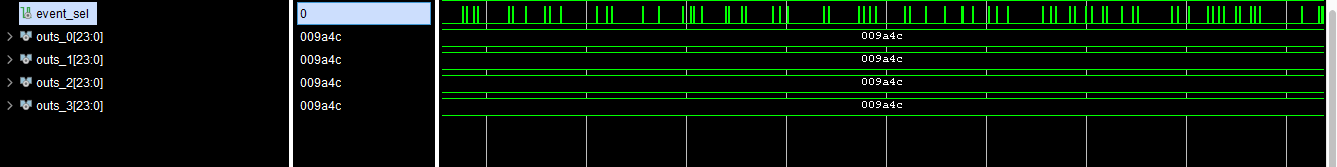
\includegraphics[width=1.00\textwidth]{gfx/diagrams/Modulo-based_coincidence_counts.png}
		\caption{The coincidence count values when a Modulo-based counter was used for random event generation (outs\_ values)} 
		\label{fig:3.9}
	\end{figure}
	
	\item \textbf{Linear Feedback Shift Register(LFSR) Implementation}
	LFSR generates a pseudo-random sequence. It is a shift register where each bit is a linear function of its previous bits, typically using XOR operations for feedback.
	
	\begin{lstlisting}
	if rising_edge(tb_clk) then
		if reset = '0' then
			Q_lfsr <= x"01";
		else
			tmp := Q_lfsr(0) XOR Q_lfsr(2) XOR Q_lfsr(3) XOR Q_lfsr(4);
			Q_lfsr <= tmp & Q_lfsr(7 downto 1);
		end if;
	end if;
	\end{lstlisting}
	
	\begin{itemize}
		\item [$\rightarrow$] \textbf{Mechanism: }
		This configuration initializes Q\_lfsr to a seed value on reset. On each clock cycle, it performs XOR operations on select bits (Q\_lfsr(0), Q\_lfsr(2), Q\_lfsr(3), and Q\_lfsr(4)) to generate the new LFSR value.
		\item [$\rightarrow$] \textbf{Purpose: }
		 LFSRs are commonly used for random signal generation due to their simple and fast implementation.
		\item [$\rightarrow$] \textbf{Result: }
		It often repeats with a fixed periodicity, which can make the randomness feel limited for event generation.	
	\end{itemize}  \clearpage
	
	\begin{figure}[htbp]
		\centering
		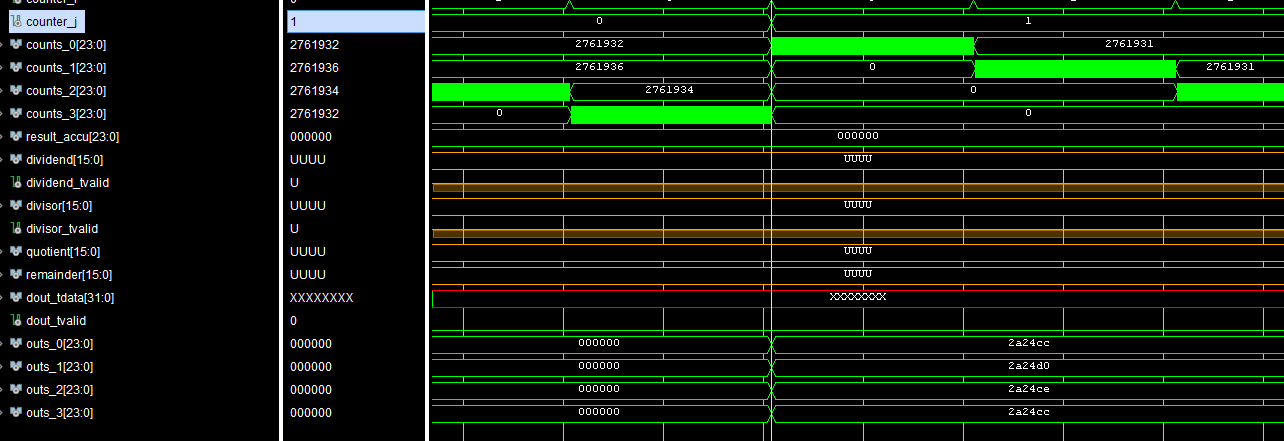
\includegraphics[width=0.85\textwidth]{gfx/diagrams/LFSR_coincidence_counts.png}
		\caption{The coincidence count values when a LFSR was used for random event generation (outs\_ / counts\_ values)} 
		\label{fig:3.10}
	\end{figure}
	
	\item \textbf{Event Occurrence Process using uniform procedure}
	This process uses the uniform procedure from IEEE.math\_real package / library, which takes in two seed values (seed1 and seed2) and produces a random real number r in the range [0, 1).
	
	\begin{itemize}
		\item [$\rightarrow$] \textbf{Mechanism: }
		In this process, uniform generates a real number r at each clock cycle. When r is above a threshold (e.g., 0.9), tb\_events is set high, simulating an event.
		\item [$\rightarrow$] \textbf{Purpose: }
		This threshold-based approach introduces randomness effectively, as r changes dynamically each cycle.
		\item [$\rightarrow$] \textbf{Result: } By setting the threshold, we control the frequency of event occurrences while keeping a natural randomness in when these events happen. This approach is generally more effective for simulating random events in digital systems. The coincidence counts showed better randomness between each other. This was needed to simulate the violation of Bell Inequality. 

	\end{itemize}

	
	\begin{figure}[htbp]
		\centering
		%\vspace{-15em}  % Adjust the value to control the amount of space reduced
		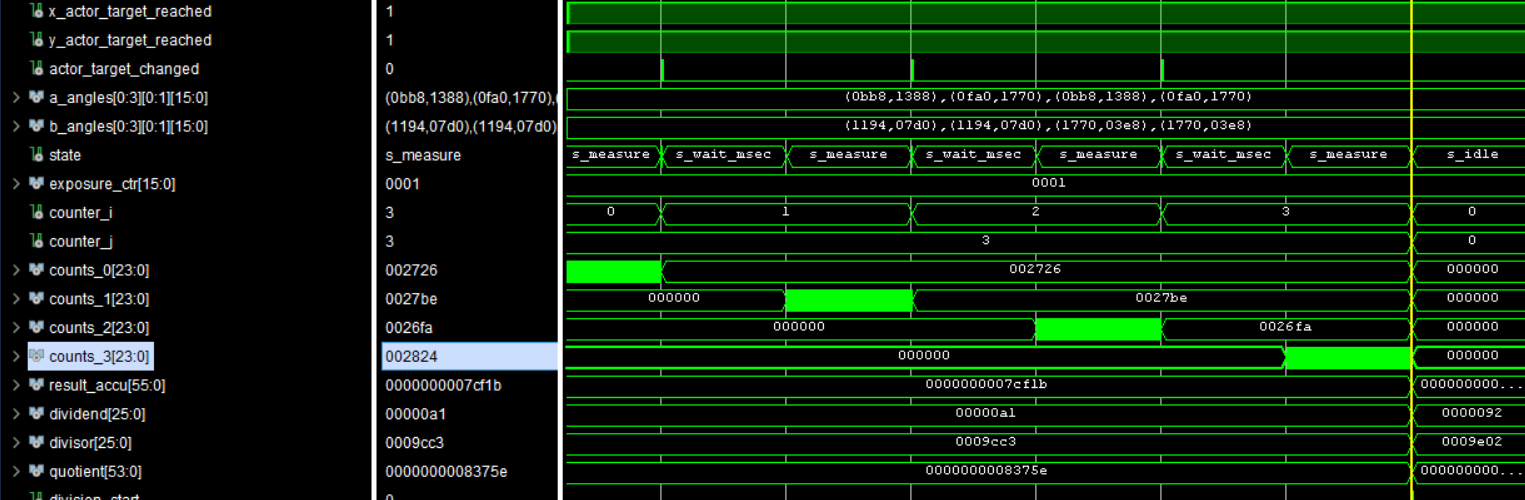
\includegraphics[width=0.85\textwidth]{gfx/diagrams/uniform_proc_coincidence_counts.png}
		\caption{The coincidence count values when a uniform procedure was used for random event generation (outs\_ values)} 
		\label{fig:3.11}
	\end{figure}
	
		
	\begin{lstlisting}
		event_occurance : process(tb_clk)
		variable r : real;
		variable seed1 : positive := 999;
		variable seed2 : positive := 999;
		begin
		if rising_edge(tb_clk) then
		uniform(seed1, seed2, r);
		if r > 0.9 then
		tb_events <= (others => '1');
		else
		tb_events <= (others => '0');
		end if;
		end if;
		end process;
	\end{lstlisting}
	
	\end{itemize}



